\begin{figure}[htbp]
 \centering
        \tikzstyle{background grid}=[draw, black!50,step=.25cm]
\tikzstyle{background grid}=[draw, black!50,step=.25cm]
	\begin{tikzpicture}[scale=1]%, show background grid]
	\tikzset{
    	mynode/.style={rectangle,rounded corners,draw=black, top color=white, bottom color=yellow!50,very thick, inner sep=0.5em, minimum size=2em, 		text centered, text width=3.3cm},
	    myarrow/.style={->, >=latex', shorten >=1pt, thick},
	    myline/.style={-, =latex', shorten >=1pt, rounded corners, ultra thick},
	    mylabel/.style={text width=7em, text centered} 
	} 
	\node[mynode] (atc) {Konwerter RS232$\Leftrightarrow$RS485 USB$\Leftrightarrow$RS485 Ethernet$\Leftrightarrow$RS485};  
	\node [left=of atc] (laptop) {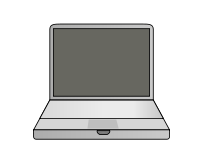
\includegraphics[width=3cm]{images/laptop}};

	\node[mynode, below=1.5cm of atc] (device2) {Urządzenie 2};
	\node[mynode, left=of device2] (device1) {Urządzenie 1};  	 	 	
	\node[mynode, right=of device2] (device12) {Urządzenie 12};	

	\draw[myline,yellow] (laptop.east) -- ++(-0.9, 0) -- (atc.west);

	\draw[myline] (atc.south) -- (device1.north); 
	\draw[myline] (atc.south) -- (device2.north); 
	\draw[myline] (atc.south) -- (device12.north); 		
	\draw[myline, dotted] (device2.east) -- (device12.west); 	
    
	\draw [fill=blue!5, thick] (-5, -5) rectangle (1, -4);

    \draw [yellow, line width=6] (-4.5,-4.5) -- (-4,-4.5); \node at (-3.5,-4.5) {USB};
    \draw [black, line width=6] (-2,-4.5) -- (-1.5,-4.5); \node at (-0.8,-4.5) {RS-485};
\end{tikzpicture} 
\caption{Topologia sieci.}
\label{elan:topologia}
\end{figure}